\section{Holographic interpretation of wormhole solutions}\label{sec:PTsym}

For wormhole solutions connecting two asymptotic AdS regions, the interpretation is that there is a Hilbert space associated to each of the boundaries and that the wormhole is an entangled state in the tensor product of the two Hilbert spaces. For an eternal black hole with asymptotic regions connected by an Einstein-Rosen bridge, the state is identified as the thermofield double state \cite{Maldacena:2001kr}. The ER bridge is not a traversable wormhole, but it can be made traversable by introducing double-trace couplings between the two boundaries \cite{Gao:2016bin}. For non-Hermitian systems, interactions may not be necessary in order to have a traversable wormhole \cite{Harper:2025lav}.  

\subsection{Pseudo-Hermiticity and \PT-symmetry}
%

In our setup we have two non-interacting copies of deformed super Yang-Mills theories. We extend analytically some of the operators and couplings in such a way that the theory is pseudo-Hermitian and \PT-symmetric for appropriately defined transformations. 

Let us consider a set of gauge-invariant operators in a representation $R$ (and its complex conjugate $\overline{R}$) of the global symmetry group, and their associated couplings
\begin{equation}
	{\cal O}_R\ ,\qquad g_R\ ;\qquad {\cal O}_{\overline{R}}\ ,\qquad g_{\overline{R}}\ .
\end{equation}
The quantum effective action of the whole system is the sum of the actions of each of the copies, one holomorphically extended to complex values and the other anti-holomorphically extended
\begin{equation}
	\Gamma=\Gamma_{SYM}\left[{\cal O}_R^{(1)},g_R=g\right]+\Gamma_{SYM}\left[\overline{{\cal O}}_{\overline{R}}^{(2)},g_{\overline{R}}=\overline{g}\right]\ .
\end{equation}
The system is pseudo-Hermitian, since there is an invertible transformation $W$ such that
\begin{equation}
\Gamma^\dagger=    W^{-1} \Gamma W\ .
\end{equation}
The transformation is\footnote{The transformation involves a transposition of the symmetry generators that changes the representation to its conjugate.}
\begin{equation}
	W: {\cal O}^{(1)}_R\to {\cal O}^{(2)}_{\overline{R}},\quad {\cal O}^{(2)}_R\to {\cal O}^{(1)}_{\overline{R}}\ .
\end{equation}
We introduce now the anti-linear transformation $T$ implementing complex conjugation
\begin{equation}
	T: {\cal O}^{(1)}_R\to \overline{{\cal O}}^{(1)}_{\overline{R}} ,\quad  {\cal O}^{(2)}_R\to \overline{{\cal O}}^{(2)}_{\overline{R}} ,\quad g\to \overline{g}\ ,
\end{equation}
and the linear transformation
\begin{equation}
	P: {\cal O}^{(1)}_R\to {\cal O}^{(2)}_R,\quad {\cal O}^{(2)}_R\to {\cal O}^{(1)}_R\ .
\end{equation}
Together, they combine in the \PT transformation
\begin{equation}
	PT: {\cal O}^{(1)}_R\to \overline{{\cal O}}^{(2)}_{\overline{R}}, \quad {\cal O}^{(2)}_R\to \overline{{\cal O}}^{(1)}_{\overline{R}},\quad g\to \overline{g}\ ,
\end{equation}
that exchanges the operators of the two copies and leaves the effective action invariant:
\begin{equation}
   (PT)^{-1}\, \Gamma\, PT=\Gamma\ .
\end{equation}
The expectation values of operators in a \PT-invariant state are related as follows
\begin{equation}
	\vev{\cO_R^{(1)}}=\bra{\Omega} \cO_R^{(1)} \ket{\Omega}=\bra{\Omega} (PT)^{-1}\cO_R^{(1)} PT\ket{\Omega}=\bra{\Omega} \overline{\cO}_{\overline{R}}^{(2)} \ket{\Omega}=\vev{\overline{\cO}_{\overline{R}}^{(2)}}=\vev{\cO_R^{(2)}}^*\ .
\end{equation}
For purely imaginary values, this implies $\vev{\cO_R^{(2)}}=-\vev{\cO_R^{(1)}}$.

In the holographic theory, we can obtain the expectation value of a scalar operator of scaling dimension $\Delta$ from the canonical momentum of the dual scalar field. The asymptotic expansion at each of the boundaries is
\begin{equation}\label{eq:asymptexp}
	\phi\underset{r\to \mp\infty}{\sim} \phi_\pm+\alpha_\pm e^{\pm(d-\Delta) r/L}+\beta_\pm e^{\pm \Delta r/L}\ ,
\end{equation}
where $\phi_\pm$ is the constant asymptotic value of the scalar. In the usual ordinary quantization the couplings $g$ for the dual operators in each copy of the field theory are proportional to the coefficients of the leading terms, $\alpha_\pm$, while the expectation values are determined by the coefficients of the subleading terms $\beta_\pm$. In the alternative quantization, the role of the coefficients is exchanged.

In ordinary quantization, $\Delta>d-\Delta$,
\begin{equation}\label{eq:vevordquant}
\begin{split}
	\vev{\cO^{(1)}}=&\ \frac{L^{d-\Delta}}{2\kappa^2_{d+1}}\lim_{r\to -\infty} e^{(d-\Delta)r/L}e^{dA}\left(\partial_r\phi-\partial_\phi W\right)\ ,\\
	\vev{\cO^{(2)}}=&\ -\frac{L^{d-\Delta}}{2\kappa^2_{d+1}}\lim_{r\to +\infty} e^{-(d-\Delta)r/L}e^{dA}\left(\partial_r\phi-\partial_\phi W\right)\ .
\end{split}
\end{equation}
The terms depending on the superpotential originate from counterterms that are introduced following the usual holographic renormalization prescription at each asymptotic boundary. Note that for BPS flows in ordinary quantization the expectation value is zero, but the formulas are valid only when the coefficient of the quadratic term in the superpotential is proportional to $d-\Delta\leq \Delta$, otherwise the leading divergences are not cancelled. For BPS flows with $\alpha_\pm=0$ the superpotential used for renormalization is different in general from the superpotential in the BPS equations, and one might find non-zero values. 

The analytic extension to imaginary values $\phi\to i\eta$ gives
\begin{equation}\label{eq:vevordquantIm}
\begin{split}
	\vev{\cO^{(1)}}=&\frac{iL^{d-\Delta}}{2\kappa^2_{d+1}}\lim_{r\to -\infty} e^{(d-\Delta)r/L}e^{dA}\left(\partial_r\eta+\partial_\eta W\right),\\
	\vev{\cO^{(2)}}=&-\frac{iL^{d-\Delta}}{2\kappa^2_{d+1}}\lim_{r\to +\infty} e^{-(d-\Delta)r/L}e^{dA}\left(\partial_r\eta+\partial_\eta W\right).
\end{split}
\end{equation}
The asymptotic expansion of $i\eta$ is the same as \eqref{eq:asymptexp}, with purely imaginary values $\phi_\pm=i \eta_\pm$, $\alpha_\pm=i \tilde\alpha_\pm$, $\beta_\pm=i\tilde\beta_\pm$.

For the flows that are not wormholes, but end at a singularity or flow to asymptotically flat spacetime, the \PT transformation exchanges solutions with the opposite sign of the superpotential. This reverses the sign of the purely imaginary expectation values of the scalars. The previous discussion would still apply to those cases, except the two copies of the theory would be in a state that factorizes.

\subsubsection{Examples}

\begin{enumerate}
	\item This is a special case where $\Delta=d-\Delta=2$, so the superpotential that cancels the divergences has the same form as the BPS superpotential, with the freedom of adding an additional finite counterterm. In the absence of sources, this implies that the expectation values vanish, so the \PT-symmetry condition is trivially satisfied 
	\begin{equation}     
	\vev{\cO^{(2)}}=-\vev{\cO^{(1)}}=0\ .
	\end{equation}
	\item In this case the field theory lives in $d=3$ dimensions. In ordinary quantization the dimension of the scalar operator would be $\Delta=2$, and the expectation values according to \eqref{eq:vevordquantIm} would be
\begin{equation}
	\vev{\cO^{(1)}}_{\Delta=2}=-\frac{i}{2\kappa_4^2} \tilde\beta_-
	\ ,\qquad
	\vev{\cO^{(2)}}_{\Delta=2}=-\frac{i}{2\kappa_4^2} \tilde\beta_+\ .
\end{equation}
However, in this case one must use alternative quantization in such a way that the dimension of the dual operator corresponds to a scalar bilinear with $\Delta=1$. This is achieved by adding a term  $\Delta {\cal L}=c\,\alpha \beta$ in the boundary action that cancels the variation with respect to the leading coefficient
\begin{equation}
\begin{split}
	\delta S_{\text{SUGRA}}=&\int \dd^dx\left(L^{\Delta_1-d}\vev{\cO}_{\Delta_1}\delta \alpha+c\delta(\alpha \beta)\right)\\
	&=\int \dd^d x\left(0 \delta \alpha+c\,\alpha\delta \beta\right)=\int \dd^d x L^{-\Delta_1}\vev{\cO}_{d-\Delta_1}\delta \beta\ .
\end{split}
\end{equation}
The expectation values are
\begin{equation}\label{eq:vevaltquant}
	\vev{\cO^{(1)}}_{\Delta=1}=\frac{i L}{2\kappa_4^2 } \tilde\alpha_-
	\ ,\qquad
	\vev{\cO^{(2)}}_{\Delta=1}=\frac{iL}{2\kappa_4^2} \tilde\alpha_+\ .
\end{equation}
The expansions of \eqref{eq:sol2} in the symmetric case $r_0=0$ give the coefficients
\begin{equation}
\begin{split}
   & \eta_-=0,\ \tilde\alpha_-=4,\ \tilde\beta_-=0\ ,\\
   & \eta_+=2\pi,\ \tilde\alpha_+=-4,\ \tilde\beta_+=0\ .
\end{split}
\end{equation}
We see that the result is consistent with the symmetric wormhole being dual to a \PT-symmetric state
\begin{equation}
	\vev{\cO^{(2)}}_{\Delta=1}=-\vev{\cO^{(1)}}_{\Delta=1}=-\frac{2iL}{\kappa_4^2}\ .
\end{equation}

\item[5.] The solution for $\eta^1$ in \eqref{eq:sol5} corresponds to introducing a mass deformation, while the solution for $\eta^2$ corresponds to an expectation value. Since the solutions are BPS, the expectation value of the operator dual to $\eta^1$ vanishes. We find that the couplings and the expectation values for each of the operators satisfy the \PT-symmetric relations
\begin{equation}
	\tilde\alpha_-^1=-\tilde\alpha_+^1=-2\sqrt{3}
	\ ,\qquad
	\vev{\cO_2^{(2)}}=-\vev{\cO_2^{(1)}}=-\frac{2i}{\kappa^2_{5}}\ .
\end{equation}

\end{enumerate}

\subsection{Entanglement between the two QFTs}

We can give a measure of the entanglement of the state dual to the wormhole by computing the mutual information between the degrees of freedom associated to each of the asymptotic AdS boundaries inside some region. 

Let us take a strip bounded by two planes separated in the $x$ direction, and compactify on a torus $T^{d-2}$ the transverse spatial directions. The entanglement entropy of the strip of 
can be computed following the Ryu-Takayangi prescription as the area of the minimal surface attached to the boundaries of a strip at each of the AdS boundaries. The full entanglement entropy of the strip taking into account all degrees of freedom corresponds to a minimal surface that is attached to both boundaries. In this case, there are two possibilities: either the minimal surface consists of two disconnected surfaces each attached to one of the boundaries, or the minimal surface connects the two boundaries through the wormhole. For the former case, the mutual information is zero, while for the latter it can be non-zero.

We will denote the area (in Planck units) of a minimal surface attached to strip A at a single boundary as $S_d(\text{A})$, and the area of the minimal surface connecting the same side of the strip at the two boundaries through the wormhole as $S_c(\text{A})$. The mutual information is
\begin{equation}
	I(\text{A})={\rm max}\,\Big\{2 \left[S_d(\text{A})-S_c(\text{A})\right],0\Big\}\ .
\end{equation}

We now proceed to compute the areas. The surface is parameterized by a profile function $x(r)$, in such a way that the induced metric on a constant time slice is
\begin{equation}
	\dd s^2
	=
	\left[1+e^{2A}(x')^2\right]\, \dd r^2+e^{2A}\dd s^2_{T^{d-2}}\ .
\end{equation}
The area in Planck units is
\begin{equation}
	S=\frac{V(T^{d-2})}{4 G_{d+1}}\int \dd r\, e^{(d-2)A}\sqrt{1+e^{2A}(x')^2}\ .
\end{equation}
Using that translations in $x$ are a symmetry, so the conjugate momentum $P$ is constant, one obtains the following equation
\begin{equation}\label{eq:solprofile}
	x'=\pm P\frac{e^{-A}}{\sqrt{e^{2(d-1)A}-P^2}}\ .
\end{equation}
Evaluating this on the area gives
\begin{equation}
S= \frac{V(T^{d-2})}{4 G_{d+1}}\int \dd r\, \frac{e^{(2d-3)A}}{\sqrt{e^{2(d-1)A}-P^2}}\ .
\end{equation}
Note that the warp factor $e^A$ reaches a minimal value at some $r=r_0$ (if the wormhole is symmetric, $r_0=0$). If $P^2< e^{2(d-1)A(r_0)}$, then the argument of the square root never vanishes and there is a profile that extends across the wormhole. This corresponds to the surfaces connecting the two boundaries. On the other hand, if $P^2> e^{2(d-1)A(r_0)}$ the profile stops at some $r_*\neq r_0$ and each of the two branches in \eqref{eq:solprofile} describes one half of a minimal surface ending at a single boundary.

We are taking the same strip on both boundaries, this means that the surfaces connecting the same side of the strip on the two boundaries should have $P=0$ for any width of the strip. On the other hand, for surfaces that are attached at a single boundary, we can characterize the profile by the value closest to the wormhole's throat that can be reached, $r=r_*$, by setting $P=e^{(d-1)A(r_*)}$. Assuming a symmetric wormhole, $r_0=0$ and $A(-r)=A(r)$, we arrive at
\begin{align}\label{eq:mutualinfstrip}
	&2 \left(S_d(\text{A})-S_c(\text{A})\right)
	=\\ &\qquad \nonumber
	\frac{V(T^{d-2})}{G_{d+1}}\left\{\int_{r_*}^\infty \dd r\, \left[\frac{e^{(2d-3)A}}{\sqrt{e^{2(d-1)A}-e^{2(d-1)A(r_*)}}}-e^{(d-2)A}\right]-\int_0^{r_*}\dd r e^{(d-2)A} \right\}\ .
\end{align}
The width of the strip is
\begin{equation}\label{eq:widthstrip}
	\Delta \ell(\text{A})=2e^{(d-1)A(r_*)}\int_{r_*}^\infty \dd r\, \frac{e^{-A}}{\sqrt{e^{2(d-1)A}-e^{2(d-1)A(r_*)}}}\ .
\end{equation}
We can show that the mutual information grows as the volume when the width of the strip is large enough. This happens when the disconnected surfaces approach each other at the wormhole's throat, $r_*\to 0$. Let us expand the warp factor around the minimum
\begin{equation}
	A(r)\sim A(0)+\frac{1}{2}A''(0) r^2\ .
\end{equation}
The leading contributions to the integrals that determine the mutual information and width are
\begin{equation}
\begin{split}
	2 (S_d(\text{A})-S_c(\text{A})) &\sim \frac{V(T^{d-2})}{G_{d+1}}e^{(d-2)A(0)}\int_{r_*}^{r_\epsilon} \dd r\, \frac{1}{\sqrt{(d-1)A''(0)(r^2-r_*^2)}}
	\ ,\\
	\Delta\ell(\text{A}) &\sim 2e^{-A(0)}\int_{r_*}^{r_\epsilon} \dd r\, \frac{1}{\sqrt{(d-1)A''(0)(r^2-r_*^2)}}\ ,
\end{split}
\end{equation}
where we have taken $r_\epsilon>r_*$ fixed and such that $A''(0)r_\epsilon^2\ll 1$. The integrals can be done analytically, and for $r_*\to 0$ they diverge as
\begin{equation}
\begin{split}
	2 (S_d(\text{A})-S_c(\text{A})) &\sim \frac{V(T^{d-2})}{G_{d+1}}\frac{e^{(d-2)A(0)}}{\sqrt{(d-1)A''(0)}}\log\frac{r_\epsilon}{r_*}
	\ ,\\
	\Delta\ell(\text{A}) &\sim 2\frac{e^{-A(0)}}{\sqrt{(d-1)A''(0)}}\log\frac{r_\epsilon}{r_*}\ .
\end{split}
\end{equation}
Thus, when the width is very large, the mutual information grows with the volume as
\begin{equation}\label{eq:mutualinfolarge}
	I(\text{A})\sim \frac{e^{(d-1)A(0)}}{2G_{d+1}}V(T^{d-2})\Delta \ell(\text{A})\ .
\end{equation}
Note that, in this limit, the factor $e^{(d-1)A(0)}V(T^{d-2})\Delta \ell(\text{A})$ becomes equal to the area of the wormhole throat at the point where the warp factor is minimal. Therefore, the amount of entanglement, as measured by the mutual information per unit volume, is determined by the `radius' of the wormhole throat. This corresponds to the saturation of the bound relating the mutual information to the entanglement wedge cross section $E_W$ \cite{Freedman:2016zud,Takayanagi:2017knl}
\begin{equation}
	E_{W}(\rho_{\text{AB}}) \geq \frac{1}{2}I(\text{A}:\text{B})\ .
\end{equation}
In our case, $\text{A}$ and $\text{B}$ correspond to the same strip on each boundary of the wormhole and $\rho_{\text{AB}}$ denotes the corresponding reduced density matrix. The holographic entanglement wedge \cite{Czech:2012bh,Wall:2012uf,Headrick:2014cta} is the region delimited by the strip on the two boundaries and the minimal surfaces that determine the entanglement entropy of $\text{A}\cup\text{B}$. The entanglement wedge cross section is defined as the minimal area that divides the entanglement wedge into two parts, each containing the strip on one of the boundaries.

\subsubsection{Examples}

For the wormhole solutions (examples 1,2 and 5 listed in subsection \ref{subsec:superpotential}), we fix the boundary metric to be Minkowski at each asymptotic AdS region. The warp factor for each case is the following:
\begin{enumerate}
\item 
Asymptotic Minkowski corresponds to $r_0=0$ and $e^{2a_0}=2$ in \eqref{eq:sol1}. The warp factor reads
\begin{equation}
	e^{2A(r)}=% generated by calc/mathematica -- do not edit
2 \cosh \left(\frac{2 r}{L}\right)
\ .
\end{equation}

\item 
Similarly, asymptotic Minkowski fixes $r_0=0$ and $e^{2a_0}=4$ in \eqref{eq:sol2} and the warp factor is
\begin{equation}
	e^{2A(r)}=% generated by calc/mathematica -- do not edit
4 \cosh ^2\left(\frac{r}{L}\right)
\ .
\end{equation}

\item[5.] 
Here the asymptotic Minkowski condition fixes $r_1=r_2=0$ and $e^{2a_0}=2^{4/3}$ in \eqref{eq:sol5}. The warp factor is
\begin{equation}
	e^{2A(r)}=% generated by calc/mathematica -- do not edit
2 \sqrt[3]{2} \cosh \left(\frac{r}{L}\right) \sqrt[3]{\cosh \left(\frac{3 r}{L}\right)}
\ .
\end{equation}

\end{enumerate}
In the three examples above, the integrals \eqref{eq:mutualinfstrip} and \eqref{eq:widthstrip} can be computed numerically upon changing the radial variable to $u=r/L$. Results are plotted in Figure~\ref{fig:mutualinfo}.
In all three cases, the mutual information presents the following features: it vanishes below a (case dependent) critical width, and it grows linearly with the width at large values. Fitting the the high $\Delta\ell$ part of the plot to a linear function, $\frac{I}{\cal{C}V}=m\cdot \frac{\Delta \ell}{L} + n$, we find for each example:
\begin{align}
	m_1 &\approx \valMISlopeExOne\,, \hspace{2.5cm} n_1 \approx \valMIInterceptExOne\,, \\
	m_2 &\approx \valMISlopeExTwo\,, \hspace{2.5cm} n_2 \approx \valMIInterceptExTwo\,, \\
	m_5 &\approx \valMISlopeExFive\,, \hspace{2.5cm} n_5 \approx \valMIInterceptExFive\,.
\end{align}
These values for the asymptotic slopes at large width agree with the formula in \eqref{eq:mutualinfolarge}.

\begin{figure}
	\centering
	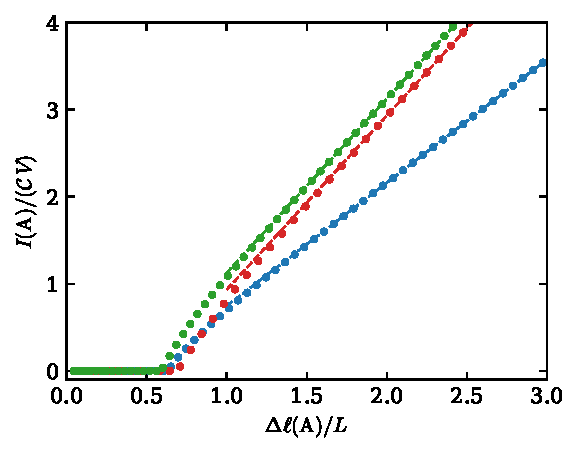
\includegraphics{mutual_information} % calc/python/scripts/04_mutual_information.py
	\caption{Mutual information of a strip $I(A)/({\cal C} V(T^{d-2}))$ as a function of the width $\Delta \ell(A)/L$, with ${\cal C}=L/G_{d+1}$. The cases represented here are the wormholes obtained from the analytic extensions of: 1. Coulomb branch of ${\cal N}=4$ SYM (blue), 2. Coulomb branch of ABJM (red), and 5. GPPZ (green). The dots are computed numerically using \eqref{eq:mutualinfstrip} and \eqref{eq:widthstrip}, and the dashed lines are linear fits at large values of the width. The slopes of the fits agree with \eqref{eq:mutualinfolarge}.}
	\label{fig:mutualinfo}
\end{figure}

\subsection{Spontaneous breaking of Poincar\'e symmetry to the diagonal group}

We have argued that the wormholes describe the low-energy limit of two stacks of branes and anti-branes that have undergone tachyon condensation. The endpoint consists of two decoupled copies of a QFT, but the wormhole is dual to a non-trivial entangled state in the product Hilbert space. 

In principle, two decoupled QFTs have two independent global Poincar\'e symmetries transforming the fields in each theory independently. We claim that the wormhole connecting the two asymptotic AdS boundaries is dual to a state that spontaneously breaks the symmetry to a diagonal symmetry $ISO(d-1,1)_1\times ISO(d-1,1)_2\to ISO(d-1,1)_D$.  The diagonal Poincar\'e symmetry is manifest in the isometries of the wormhole solution, and we show that there is a Goldstone corresponding to the broken symmetry. Similar arguments have been made for Euclidean wormholes in \cite{Betzios:2023obs}, building on the solutions  \cite{Betzios:2019rds,Betzios:2021fnm}.

As we already mentioned, the non-gravitational analog of a wormhole provided by the connected D8-anti D8 brane configuration in the Sakai-Sugimoto model corresponds to the spontaneous breaking of left and right chiral flavor symmetries to the diagonal vector symmetry $U(N_f)_L\times U(N_f)_R\to U(N_f)_V$, where $N_f$ is the number of flavors. Let us review in more detail how the holographic dictionary works in that example, as we employ it to inform our interpretation of the gravitational wormholes.

We denote $z$ as the radial holographic coordinate along the D8 brane worldvolume, such that the asymptotic boundaries are at $z\to \pm\infty$. On the connected D8 branes, there is a $U(N_f)$ gauge field. Sources for the global currents associated to each of the chiral flavor symmetries, $l_\mu$ and $r_\mu$, map, in the holographic dual, to the asymptotic values of the gauge field:
\begin{equation}
	\lim_{z\to-\infty} A_\mu(z,x)=l_\mu(x)
	\ ,\qquad 
	\lim_{z\to+\infty} A_\mu(z,x)=r_\mu(x)\ .
\end{equation}
Similarly, the expectation values of the chiral flavor currents can be obtained from the coefficients of the subleading terms in the asymptotic expansions of $A_\mu$ at each of the boundaries. The solutions for the gauge field split according to their parity in the $z$ direction. Parity-even solutions correspond to the vector sector, while parity-odd solutions correspond to the axial sector, the former being symmetric with respect to swapping left and right chiralities while the latter is antisymmetric. 

Proper gauge transformations in the D8 brane worldvolume are those vanishing at the boundaries. On the other hand, while gauge transformations that asymptote to a constant correspond to global symmetry transformations in the dual field theory, general gauge transformations that do not vanish at the boundary correspond to background gauge field transformations of the sources. 

Let us focus on the case where the gauge field vanishes in the background D8 brane solution and we look at linearized fluctuations around this background. The linearized gauge transformations are
\begin{equation}
	\delta A_M=\partial_M \lambda\ .
\end{equation}
We can introuduce a Wilson line, invariant under proper gauge transformations, that connects the two boundaries 
\begin{equation}
     W(x)=\int_{-\infty}^\infty \dd z\, A_z(z,x)\ .
\end{equation}
For general gauge transformations, the Wilson line transforms as expected for a Goldstone boson of the broken axial symmetry
\begin{equation}
	\delta W(x)=\lim_{z\to +\infty} \lambda-\lim_{z\to-\infty} \lambda=\lambda_R-\lambda_L
	\ .
\end{equation}
By solving the equations of motion for fluctuations on the brane, one finds that indeed there is a massless mode making the Wilson line non-zero.

Let us now move on to the gravitational wormhole and show that there is a Goldstone associated with the broken Poincar\'e symmetry analogous to the Goldstone of the flavor symmetries of the D8 branes in the Sakai-Sugimoto model. The holographic radial coordinate is now denoted as $r$, with the asymptotic AdS boundaries at $r\to \pm\infty$.

In this case, we are interested in the metric. We could couple each of the dual QFTs to a different background metric, which would map to the asymptotic value of the metric in the gravity dual at the boundaries,
\begin{equation}
	\lim_{r\to-\infty} g_{\mu\nu}(r,z)\sim e^{-2r/L}g^{(0),[1]}_{\mu\nu}(x)
	\ ,\qquad
	\lim_{r\to+\infty} g_{\mu\nu}(r,z)\sim e^{2r/L}g^{(0),[2]}_{\mu\nu}(x)\ .
\end{equation}
The subleading terms in the asymptotic expansion at each boundary determine the expectation values of the energy momentum tensors in each of the QFTs. Following the example of the Sakai-Sugimoto model, if we classify solutions according to their parity with respect to the $r\to -r$ transformation, parity-even solutions should correspond to the sector of operators arranged in representations the diagonal Poincar\'e subgroup and parity-odd solutions to the sector corresponding to the antidiagonal subgroup. 

The gauge symmetry associated to the metric are diffeomorphisms. 
We describe the background wormhole metric in domain wall coordinates
\begin{equation}
	\dd s^2
	=
	\dd r^2+e^{2A(r)}\eta_{\mu\nu}\,\dd x^\mu \dd x^\nu\ ,
\end{equation}
and expand the metric in background plus linear fluctuations
\begin{equation}
	G_{MN}=g_{MN}+h_{MN}\ .
\end{equation}
In the following, we do not enforce any gauge condition. Imposing the radial gauge would eliminate the components that capture the Goldstone mode.

Linearized diffeomorphisms transform the metric components as (indices are lowered with the Minkowski metric)
\begin{eqnarray}
	\delta h_{\mu\nu}&=&-2e^{2A}\partial_{(\mu}\xi_{\nu)}-2A'e^{2A}\eta_{\mu\nu}\xi^r\ ,\\
	\delta h_{\mu r} &=& -e^{2A}\partial_r \xi_\mu-\partial_\mu \xi^r\ ,\\
	\delta h_{rr} &=& -2\partial_r\xi^r\ .
\end{eqnarray}
We study vector fluctuations of the metric components $h_{\mu r}$ around the background. The other components are invariant under a subset of the diffeomorphisms satisfying
\begin{equation}\label{eq:alloweddiff}
     \xi^r=0
     \ ,\qquad \partial_{(\mu}\xi_{\nu)}=0
     \ .
\end{equation}
Thus, for each fixed value of $r$, $\xi^\mu(r,x)$ is a Killing vector of the Minkowski metric, which includes the generators of spacetime translations and Lorentz transformations,
\begin{equation}
	\xi_\mu=c_\mu+\omega_{\mu\nu} x^\nu
	\ ,\qquad
	\omega_{\mu\nu}=-\omega_{\nu\mu}\ .
\end{equation}
We consider the transverse vector component of the metric 
\begin{equation}
	H^\mu=-g^{\mu\alpha}h_{\alpha r}^t
	\ ,\qquad 
	\partial^\mu h_{\mu r}^t=0\ .
\end{equation}
Under linearized diffeomorphisms satisfying \eqref{eq:alloweddiff}, it transforms as
\begin{equation}
	\delta H^\mu=\partial_r \xi^{t\,\mu}
	\ ,\qquad
	\partial_\mu \xi^{t\,\mu}=0\ . 
\end{equation}
Note that the allowed diffeomorphisms \eqref{eq:alloweddiff} automatically satisfy the transverse condition, so we will drop the label below.

The analog to the Wilson line for translations is
\begin{equation}\label{eq:Wm}
	W^\mu(x)=\int_{-\infty}^\infty \dd r\, H^\mu(r,x)\ .
\end{equation}
Its transformation under diffeomorphisms is 
\begin{equation}
	\delta W^\mu=\lim_{r\to +\infty} \xi^\mu -\lim_{r\to -\infty} \xi^\mu\ .
\end{equation}
This is consistent with $W^\mu$ transforming as the Goldstone boson of the broken antidiagonal Poincar\'e symmetry, particularly translations. For Lorentz transformations we can introduce
\begin{equation}
	W_{\alpha\beta}(x)=2\partial_{[\alpha} W_{\beta]}(x)\ ,
\end{equation}
that transforms as expected for the Goldstones of the broken antidiagonal Lorentz symmetry
\begin{equation}
	\delta W_{\alpha\beta}=\lim_{r\to +\infty} 2\partial_{[\alpha}\xi_{\beta]} -\lim_{r\to -\infty} 2\partial_{[\alpha}\xi_{\beta]}\ .
\end{equation}
As usual, these are not independent from the Goldstones of broken translations \cite{Low:2001bw}.

Setting $h_{rr}=0$ and $h_{\mu\nu}=0$,
the linearized equations of motion for the vector metric fluctuation are
\begin{subequations}
\begin{eqnarray}
     \partial^2 h_{\mu r} &= &0\ ,\\
	\partial^\mu h_{\mu r} &= &0\ ,\\
     \partial_r \left(e^{(d-2)A} \partial_{(\mu} h_{\nu) r}\right) &=&0\ .
\end{eqnarray}
\end{subequations}
The first two equations correspond to a massless transverse vector mode along the Minkowski directions. From the last equation we obtain the radial dependence
\begin{equation}
	h_{\mu r}(r,x)=v_\mu(x) e^{-(d-2) A(r)}\ .
\end{equation}
This is a normalizable mode at both boundaries, in such a way that \eqref{eq:Wm} is finite. We can then identify this mode with the Goldstone for the broken antidiagonal Poincar\'e symmetry.

